\title{CFD laboratory 1\\Laminar flow development between two parallel plates}
\author{
        Sergio M. Vanegas A.\\
        Francesco de Pas\\
                Department of Mathematics\\
        Polimi---Politecnico di Milano\\
        Milano, Italia
}
\date{\today}

\documentclass[12pt]{article}

\usepackage{amsmath}
\usepackage{graphicx}

\begin{document}
\maketitle

\begin{abstract} 
 The fourth test case is the flow around a circular cylinder in the sub-critical regime. The cylinder is considered with infinite height to avoid side effects. The flow develops from the free-stream profile \mathcal {U} _ \infty in the form of a laminar boundary layer that, after separation at about 82° from the leading edge, generates a turbulent wake with some periodic behavior. The phenomenon is inherently unsteady even at the macro-scale and therefore it requires solving the U-RANS, which might be computationally demanding even for a 2D problem. As a consequence it is here performed the grid independence study for a steady state (RANS) model, and then use the same grid settings for the subsequent U-RANS simulation.\cite{FL:01}
\end{abstract}

\section{Introduction}

In the sub-critical regime, the laminar boundary layer developing over the walls of the cylinder separates at about 82° from the front stagnation point, and a large, turbulent wake generates downstream. The pressure distribution over the walls of the cylinder, shown in Figure 2 (ADD FIGURE), agrees with the potential flow solution only in the front part of the body. The separation point is just at the beginning of the region of adverse pressure gradient, and it can be easily recognized in the figure since the wall pressure in the wake region is broadly uniform. Additionally, the wall shear stress is zero at the point of separation.
The drag coefficient of a circular cylinder with infinite length is defined as: ADD FORMULA and it is a function of 𝑅𝑒𝐷 and the relative roughness 𝑠/𝐷𝐶. In the sub-critical regime, 𝐶𝐷 is nearly constant with 𝑅𝑒𝐷, and it is not much affected by the roughness. Such constant value is around 1.2, as is it evident from the plot below (Figure 3 ADD FIGURE 3).
Finally, the dimensionless Strouhal number quantifies the characteristic frequency of the turbulent wake, 𝑓,and it is defined as 𝑆𝑡 = 𝑓𝐷𝐶/𝑈∞. The paper by Fey et al. (1998) provides a correlation to estimate 𝑆𝑡 as a function of 𝑅𝑒𝐷, according to which, in the sub-critical regime, 𝑆𝑡 varies between 0.185 and 0.21 (Figure 4 ADD FIGURE4).


        The configuration of the problem is as follows:
        \begin{itemize}
                \item Diameter \( D_c = 0.06 \: m \),
                \item Free-stream velocity \( U_\infty = 0.4 \: m/s \),
                \item Bulk velocity \( U_b = 5 \: mm/s \),
                \item Fluid: Water at \( 20^{\circ}C \; ( \rho = 998.23 \: kg/m^3\), \\ Kinematic Viscosity \( \nu = 1.006E-6 \: m^2/s ) \).
        \end{itemize}


        \paragraph{Outline}
        The remainder of the report is organized as follows: Section~\ref{sec:Steady-state precursor} provides some suitable results concerning grid independence study performed on RANS solutions; Section~\ref{sec:URAN} instead makes use of URANS in order to focus on the temporal evolution  of the process; Section~\ref{sec:Comparison with Literature} compares the results obtained with literature ones and finally  Section~\ref{sec:Comparison RANS vs URANS} compares RANS and URANS solutions, taking into account the inviscid flow potential solutions
        
      
      
\section{Steady-state precursor} \label{sec:Steady-state precursor}

The following Grid-Independence study is applied on RANS solution.   Despite in principle RANS solutions do not provide a trustful representation of the physical phenomenon under investigation, this choice can been consider a practical compromise to face the heavy URANS  computational cost. The variables under investigation are:  the distributions of wall pressure and wall shear stress, the drag coefficient and the position of the separation point, inferred from the wall pressure and the wall shear stresses.In particular the separation point was inferred by the wall pressure approximating the wall pressure second derivative (through finite differences of order 8) and looking for its inflection point. The separation point was instead inferred by the shear stress imposing it as the shear stress zero.
The study was performed by fixing BOH QUANTE and then progressively increasing the number of slices in which our domain was cut.
Figure~\ref{fig:drag_independence},Figure~\ref{fig:pression_ind},Figure~\ref{fig:wall_ind}show our results.
        \begin{figure}[!ht]
                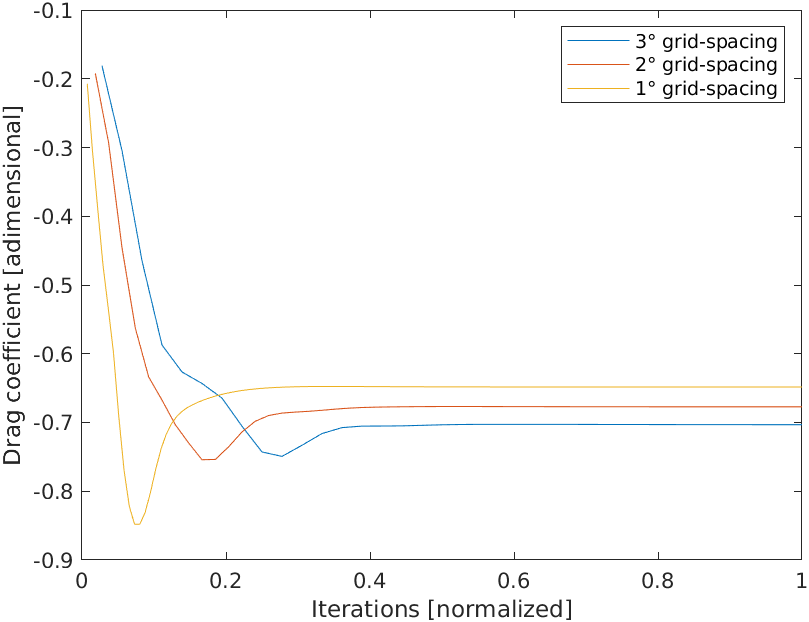
\includegraphics[width=\textwidth]{DragCoefficient_Independence.png}
                \centering
                \caption{}
                \label{fig:drag_independence}
        \end{figure}

        \begin{figure}[!ht]
                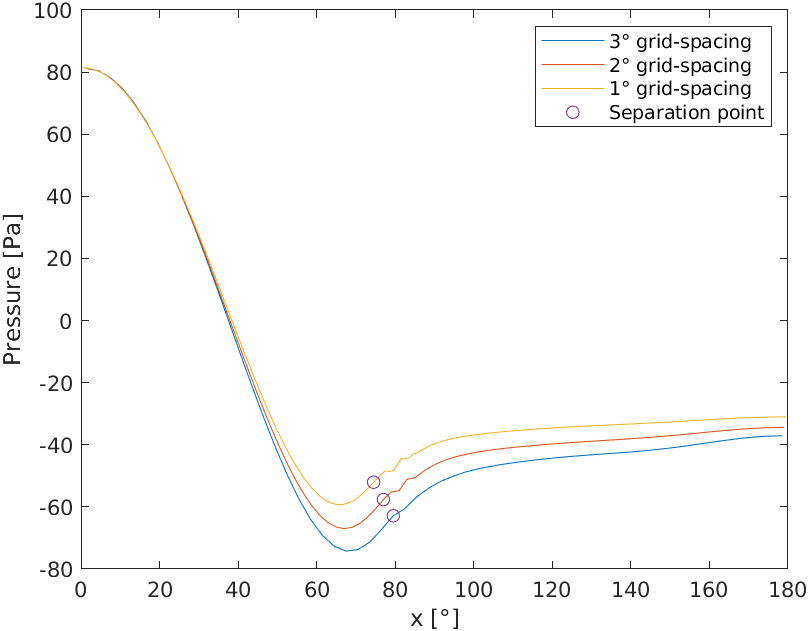
\includegraphics[width=\textwidth]{Pressure_Independence.png}
                \centering
                \caption{}
                \label{fig:pression_ind}
        \end{figure}

        \begin{figure}[!ht]
                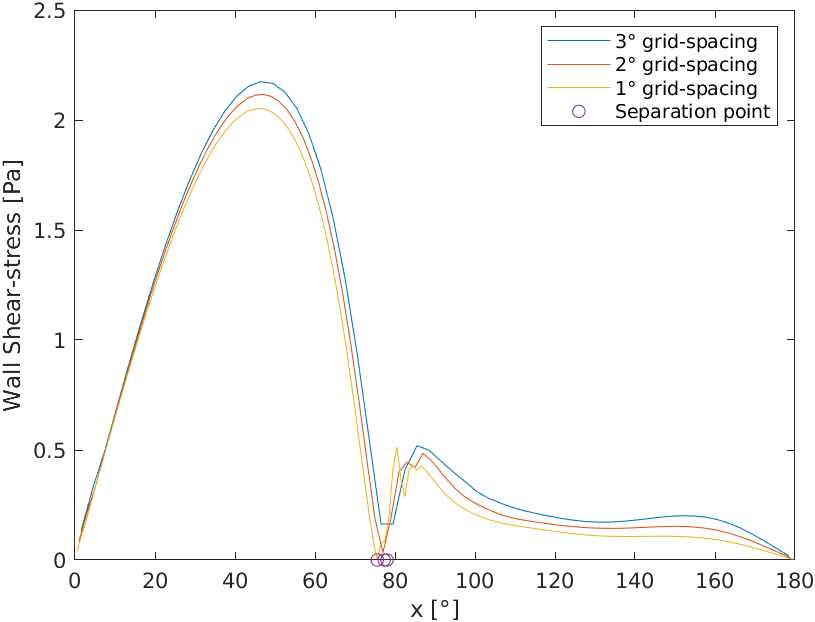
\includegraphics[width=\textwidth]{WallShearStress_Independence.png}
                \centering
                \caption{X-velocity Y-profile per delta-step}
                \label{fig:wall_ind}
        \end{figure}


According to experimental results separation point s should lie at $$ 82 ^\circ $$, and our plot quite respect this result.

\section{Unsteady-state modelling} \label{sec:URAN}
In this section we'll make use of our results from URANS simulations. To launch these simulations we re-started from the converged steady-state solutions exploiting the same grid settings.
We defined as suitable total simulation time to observe periodicity in the macroscopic flow NON LO SO.
Then we performed a sensibility analysis with respect to the time-step of time discretization, considering as target parameters NON LO SO.
Then we decided to consider the vector of drag and lift forces measured each \textit{6ms}, i.e. we focused on a frequency of \mathcol{1\6 [s^{-1}]}, and their temporal evolution can be seen in Figure~\ref{fig:drag} and Figure~\ref{fig:lift}. This results are well aligned with the process dynamic since we expect the turbolent wake to strongly affect lift oscillations mantaining its mean null over time, while not causing visibly drag force oscillations since it does not create any counter flow.
As it can be seen in figure ADD the amplitude of drag force signal is of the order of \mathcol{1*10^{-4}}, and its frequency of \mathcol{1*10^{-1}}, while for the lift force signal both its amplitude is of order \mathcol{10^-3} while its frequency are of order \mathcol{1}. 
To compare its frequences watch figure (ADD) where fluctuating Lift has been raised of \textit{<Cd>=0.993}, it is clear that drag signal has one order of magnitude less amplitude and frequencies. They seems to be in PHASE OR NOT BOH

        \begin{figure}[!ht]
                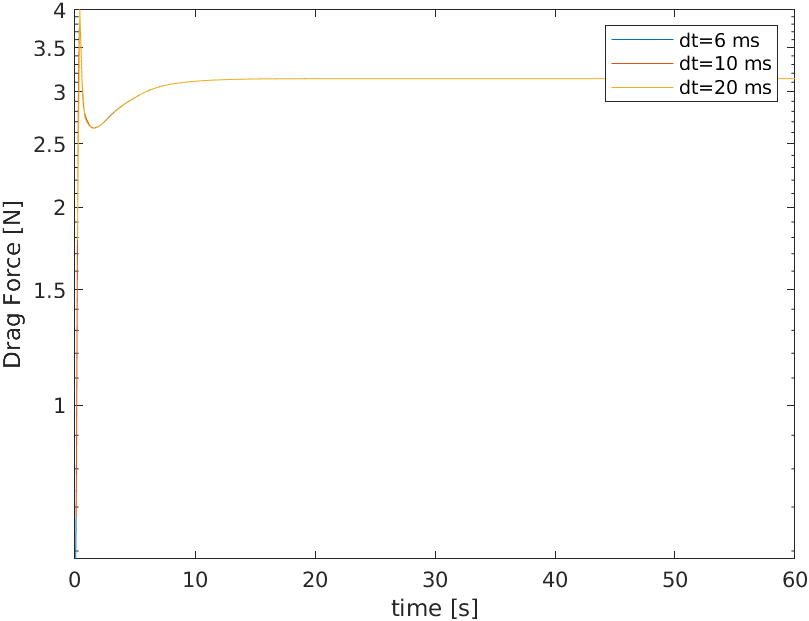
\includegraphics[width=\textwidth]{DragForce.png}
                \centering
                \caption{}
                \label{fig:drag}
        \end{figure}

        \begin{figure}[!ht]
                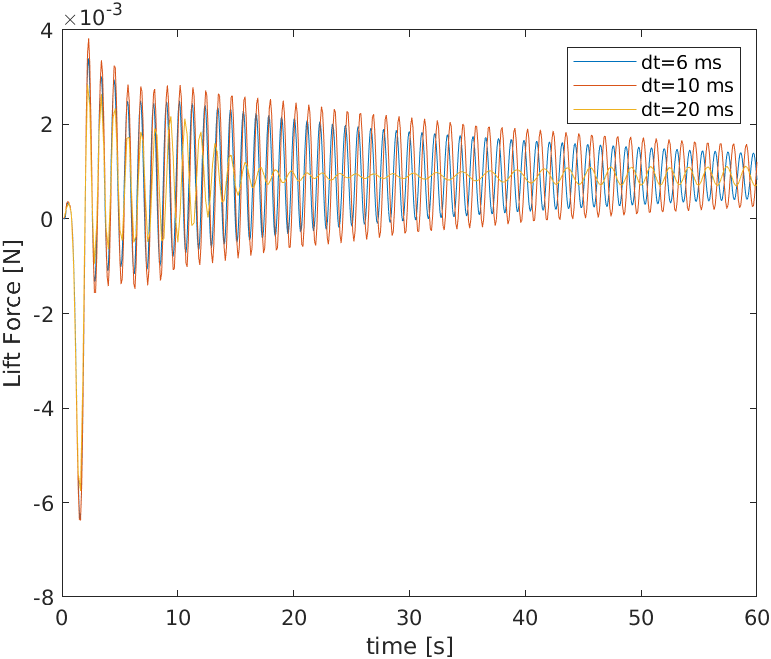
\includegraphics[width=\textwidth]{LiftForce.png}
                \centering
                \caption{}
                \label{fig:lift}
        \end{figure}
        
Then we calculated the time-averaged drag coefficient from the U-RANS simulation, reported in figure Figure~\ref{fig:coeff}. According to reference it should be 1.2 for us it is 0.6
        \begin{figure}[!ht]
                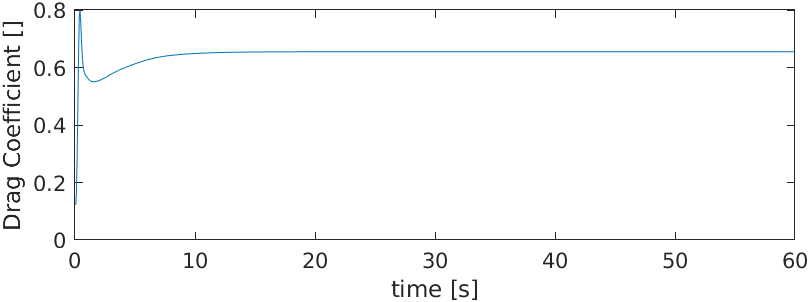
\includegraphics[width=\textwidth]{Coefficients.png}
                \centering
                \caption{}
                \label{fig:coeff}
        \end{figure}
        
Finally the Strohal number, since we are in subcritical regime should be between 0.185 and 0.21




















\bibliographystyle{abbrv}
\bibliography{main}

\end{document}
